\newpage
\thispagestyle{empty}
\fontsize{12pt}{13pt}\selectfont
\begin{center}\label{zhixie}
	{\xiaoerhao\textbf{致~~~~谢}}
\end{center}

\begin{flushleft}
\setlength{\parindent}{2em}
\hspace{1.6em}
% 虽然写论文的过程一直都是绝望阴暗的,但写到致谢部分已经变成希望明快的了。
我在此向所有在我硕士论文完成过程中提供支持和帮助的人们致以诚挚的感谢和敬意。

首先,我要向我的导师孙小军教授表达最真挚的感谢之情。导师不仅在研究过程中给予我专业而精准的指导和建议,更是以身作则,教会我如何做一个有追求、有担当的科研工作者。导师在我人生道路上的指引和支持,将成为我前行的力量和动力,使我更加坚定迈向未来的信心和决心。

其次,我要感谢罗秋莲等计算物理组的师兄师姐们,感谢他们在我研一时的帮助和支持。我还要感谢我的同门彭海圆师兄,梁艳师姐,张凯师兄,蓝秀丽师姐,邹方磊,唐诺程,崔嫣然,曹寒梅。另外,我还要感谢姚红师兄,万梦婷,杨赟,张国峰,陈立欣,陈叶若溪,李文琳,莫腾欢等核组的同学,我研究生大部分时间都是和他们一起度过的。以上这些人为我提供了最基础、最实用的技术支持,让我可以在学术中尽情发挥。他们严谨的治学态度、乐观向上的精神,都在潜移默化中影响和鼓励着我。

此外,我要感谢我的家人和朋友们,感谢他们在我完成学业的道路上给予我物质上的鼓励和支持。正是有了你们的陪伴和支持,我才有了追求知识和实现梦想的勇气和动力。谢谢你们的默默付出,是你们的陪伴,让我更坚定地走向自己的梦想之路。

另外,我要感谢一只特别的小生命——薛咪。她是我在研究生期间被收养的一只流浪猫。她的出现给了我无穷的欢乐和慰藉。
% 这张照片是薛咪在监督我写程序。
% \begin{figure*}[htbp]
% 	\centering
% 	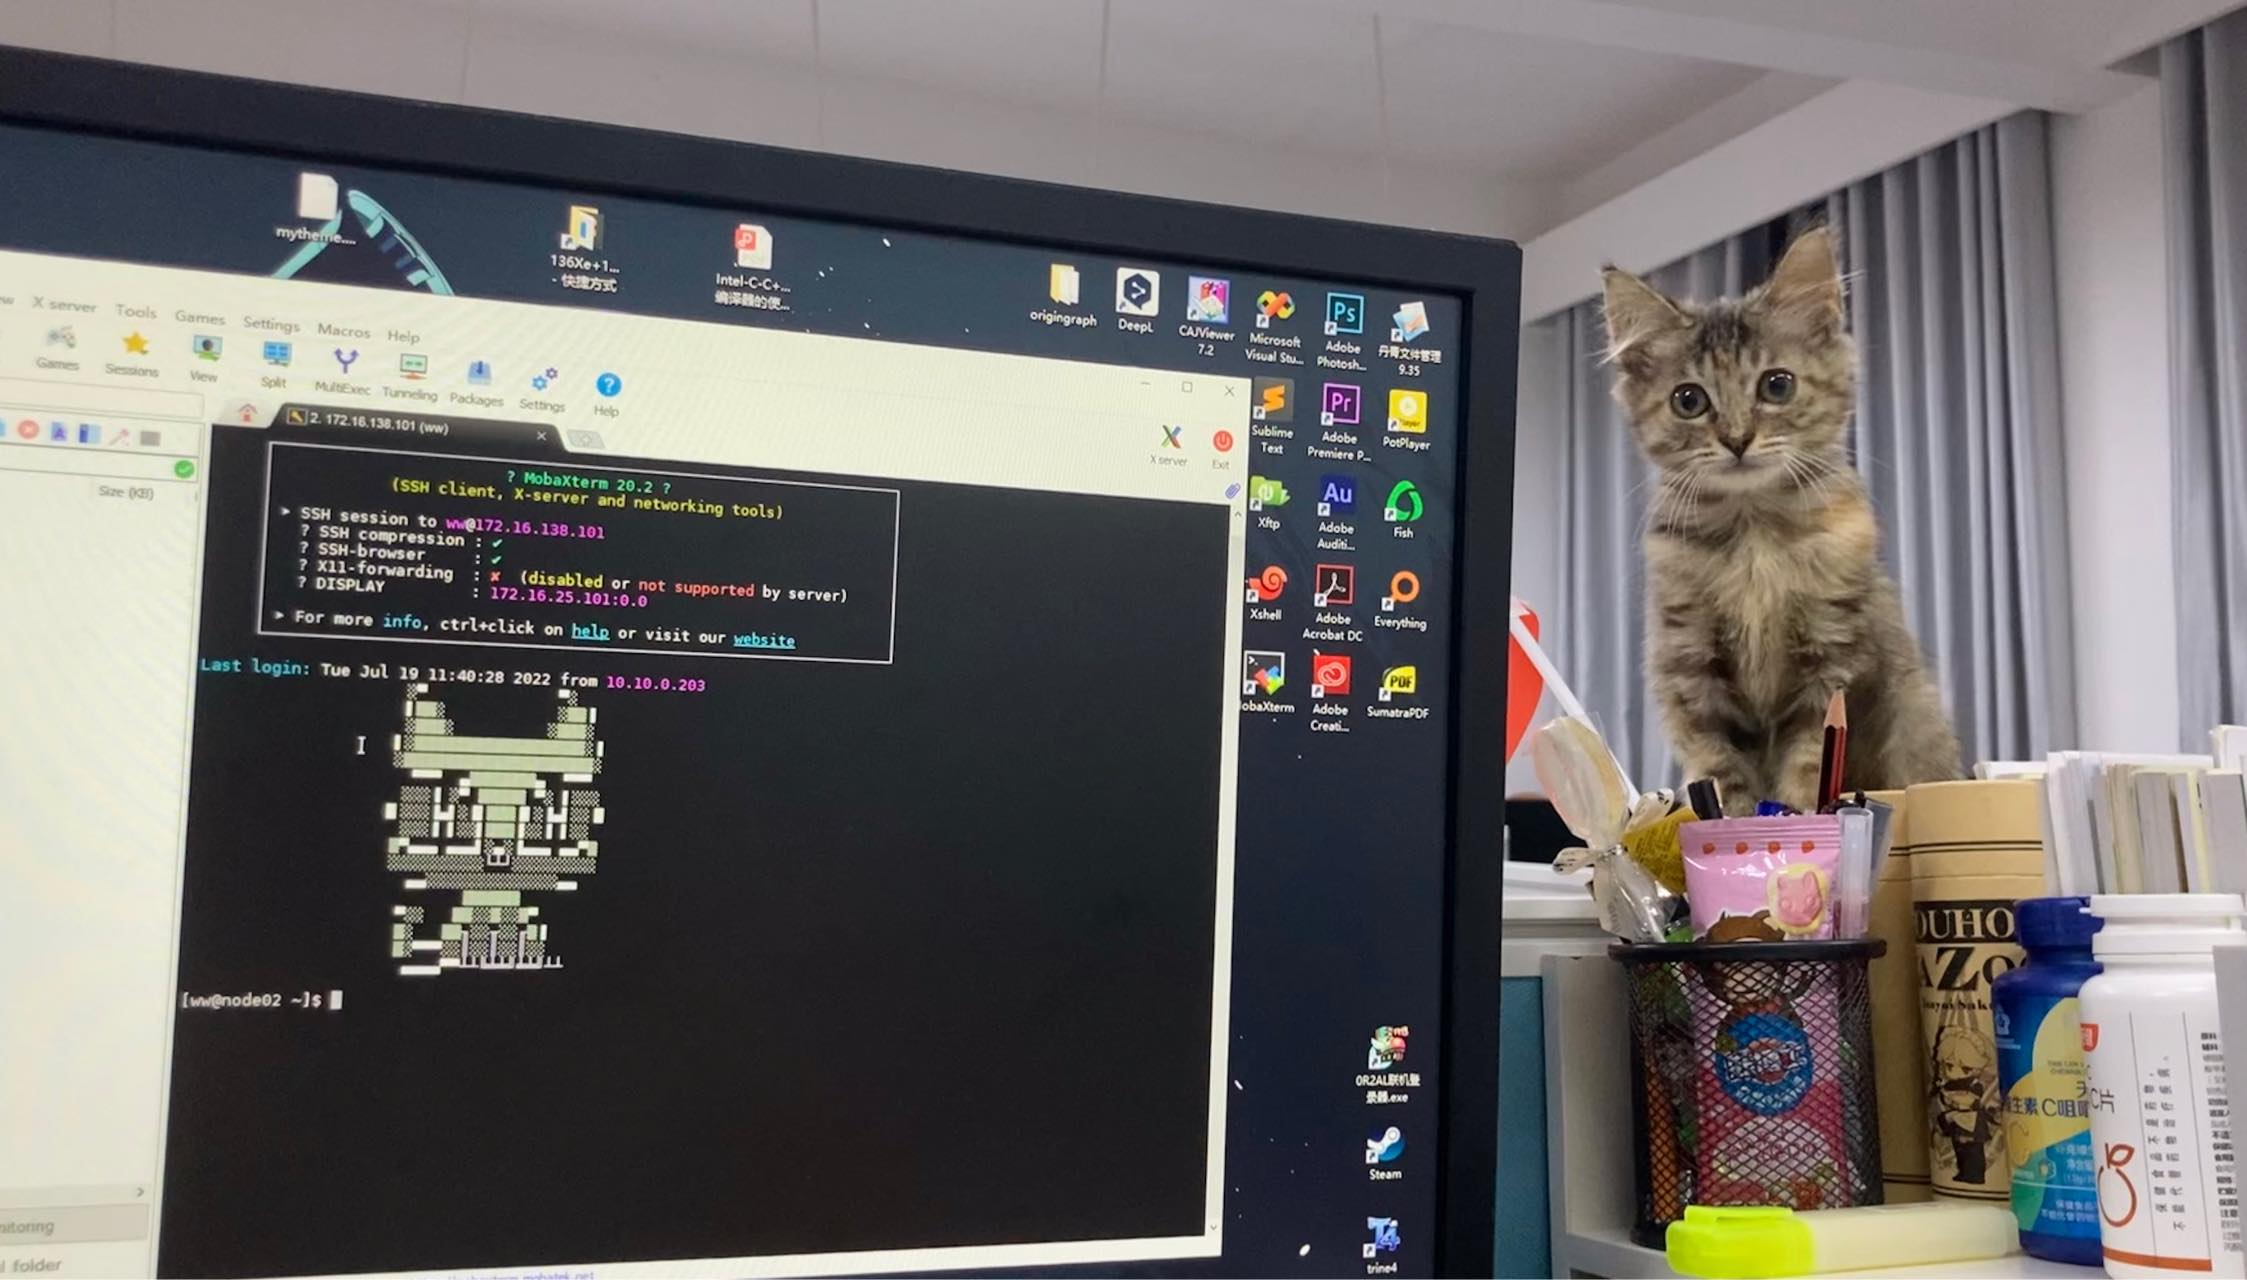
\includegraphics[width=0.76\linewidth]{figures/xuemi.jpg}
% 	% \caption{}
% 	\label{xuemi}
% \end{figure*}

最后,感谢当年选择物理专业的那个自己。一路走来,世界很美好。
\end{flushleft}


